\documentclass[11pt,a4paper]{article}
%%%----------------------------------------------------------------------------%%%
%%%----------------------------------------------------------------------------%%%
%%% 
%%% ### Packages 
%%%
%%%----------------------------------------------------------------------------%%%
%%%----------------------------------------------------------------------------%%%
\usepackage{amsmath, amsthm, amssymb, nccbbb, bm, dsfont, pifont, fontawesome, graphicx, varioref, bbold, setspace, enumitem,colortbl,mdframed,caption2,mathtools}
\usepackage{algorithm,algorithmic}
\usepackage{tikz}
\usepackage{pgfplots}
\usetikzlibrary{patterns}
\RequirePackage[round,authoryear]{natbib}
\RequirePackage[colorlinks,citecolor=red,urlcolor=red]{hyperref}
\usepackage[cal=boondox]{mathalfa}
\setlength{\topmargin}{-1in}
\setlength{\textheight}{10.5in}
\setlength{\oddsidemargin}{-.6in}
\setlength{\textwidth}{7.5in}
\hypersetup{colorlinks=true, linkcolor=myblue, citecolor=myblue, urlcolor=myblue}
\linespread{.9}
\setlist[itemize]{itemsep=0cm}
\setlist[enumerate]{itemsep=0cm}

%%%----------------------------------------------------------------------------%%%
%%%----------------------------------------------------------------------------%%%
%%% 
%%% ### Code 
%%%
%%%----------------------------------------------------------------------------%%%
%%%----------------------------------------------------------------------------%%%
\usepackage{listings}
\lstset{escapeinside=| |}
%\usepackage[usenames,dvipsnames]{color}  
\definecolor{mygray}{RGB}{242,242,242}
\definecolor{myblue}{rgb}{0.0, 0.23, 0.63}
\definecolor{myred}{rgb}{0.75, 0.0, 0.0}
\definecolor{mygreen}{rgb}{0.4, 0.69, 0.2}  
\definecolor{mypalegreen}{rgb}{0.6, 1.0, 0.6}
\definecolor{gray2}{RGB}{128,128,128} 
\definecolor{blue2}{RGB}{0,47,167}
\lstnewenvironment{R}{\lstset{ 
  language=R,
  basicstyle=\footnotesize\ttfamily, 
  numbers=left,
  numberstyle=\tiny\color{black},
  stepnumber=1,
  numbersep=5pt,
  backgroundcolor=\color{mygray},
  showspaces=false, 
  showstringspaces=false,
  showtabs=false, 
  frame=single,  
  rulecolor=\color{black},
  tabsize=4,
  captionpos=b,
  breaklines=true,
  breakatwhitespace=false,
  keywordstyle=\ttfamily\bfseries\color{myblue},
  commentstyle=\ttfamily\bfseries\color{myred},
  stringstyle=\ttfamily\bfseries\color{mygreen}
} 
}{}

\lstnewenvironment{tex}{\lstset{ 
  language=tex,
  basicstyle=\footnotesize\ttfamily, 
  numbers=left,
  numberstyle=\tiny\color{black},
  stepnumber=1,
  numbersep=5pt,
  backgroundcolor=\color{mygray},
  showspaces=false, 
  showstringspaces=false,
  showtabs=false, 
  frame=single,  
  rulecolor=\color{black},
  tabsize=4,
  captionpos=b,
  breaklines=true,
  breakatwhitespace=false,
  keywordstyle=\ttfamily\bfseries\color{myblue},
  commentstyle=\ttfamily\bfseries\color{myred},
  stringstyle=\ttfamily\bfseries\color{mygreen}
} 
}{}

%%%----------------------------------------------------------------------------%%%
%%%----------------------------------------------------------------------------%%%
%%% 
%%% ### Box
%%%
%%%----------------------------------------------------------------------------%%%
%%%----------------------------------------------------------------------------%%%

\usepackage{tcolorbox}
\tcbuselibrary{breakable}
% Custom box definition with margins migrated from md environment
\newtcolorbox{redbox}{
  colback=myred!3,      % Background color of the box
  colframe=myred,    % Border color of the box  
  leftrule=4pt,             % Thickness of the left border
  toprule=1pt,              % No top border
  bottomrule=1pt,           % No bottom border
  rightrule=1pt,            % No right border
  arc=1.2mm,                  % Rounded corners
  outer arc=1.5mm,            % Outer border radius
}


\newtcolorbox{bluebox}{
  colback=myblue!3,      % Background color of the box
  colframe=myblue,    % Border color of the box  
  leftrule=4pt,             % Thickness of the left border
  toprule=0pt,              % No top border
  bottomrule=0pt,           % No bottom border
  rightrule=0pt,            % No right border
  arc=1.2mm,                  % Rounded corners
  outer arc=1.5mm,            % Outer border radius
}

\newtcolorbox{greenbox}{
  colback=mygreen!3,      % Background color of the box
  colframe=mygreen,    % Border color of the box  
  leftrule=4pt,             % Thickness of the left border
  toprule=0pt,              % No top border
  bottomrule=0pt,           % No bottom border
  rightrule=0pt,            % No right border
  arc=1.2mm,                  % Rounded corners
  outer arc=1.5mm,            % Outer border radius
}

\newtcolorbox{graybox}{
  colback=gray2!3,      % Background color of the box
  colframe=gray2,    % Border color of the box  
  leftrule=4pt,             % Thickness of the left border
  toprule=0pt,              % No top border
  bottomrule=0pt,           % No bottom border
  rightrule=0pt,            % No right border
  arc=1.2mm,                  % Rounded corners
  outer arc=1.5mm,            % Outer border radius
}



%\newtcolorbox{mybox}{colback=yellow!5!white, colframe=gray!60!black, breakable}
\newcommand{\Solution}{\noindent{\color{myblue}{ \textsc{Solution}:~$\Big.$}}}
\newenvironment{sol}
{\Solution \par }{}


\AtBeginEnvironment{definition}{\begin{redbox} }
\AtEndEnvironment{definition}{\end{redbox}}	

\AtBeginEnvironment{proposition}{\begin{redbox} }
\AtEndEnvironment{proposition}{\end{redbox}}	

\AtBeginEnvironment{lemma}{\begin{redbox} }
\AtEndEnvironment{lemma}{\end{redbox}}	
\AtBeginEnvironment{theorem}{\begin{redbox} }
\AtEndEnvironment{theorem}{\end{redbox}}	

\AtBeginEnvironment{corollary}{\begin{redbox} }
\AtEndEnvironment{corollary}{\end{redbox}}	
\AtBeginEnvironment{condition}{\begin{redbox} }
\AtEndEnvironment{condition}{\end{redbox}}	

\AtBeginEnvironment{remark}{\begin{graybox} }
\AtEndEnvironment{remark}{\end{graybox}}	

\AtBeginEnvironment{example}{\begin{bluebox} }
\AtEndEnvironment{example}{\end{bluebox}}	

\AtBeginEnvironment{exercise}{\begin{bluebox} }
\AtEndEnvironment{exercise}{\end{bluebox}}	

\AtBeginEnvironment{question}{\begin{bluebox} }
\AtEndEnvironment{question}{\end{bluebox}}	





%%%----------------------------------------------------------------------------%%%
%%%----------------------------------------------------------------------------%%%
%%% 
%%% ### Theorem style structures 
%%%
%%%----------------------------------------------------------------------------%%%
%%%----------------------------------------------------------------------------%%%

\numberwithin{equation}{section}
\theoremstyle{plain}
\newtheorem{theorem}{Theorem}[section]
\newtheorem{lemma}[theorem]{Lemma}
\newtheorem{corollary}[theorem]{Corollary}
\newtheorem{proposition}[theorem]{Proposition}
\newtheorem{condition}{Condition}[section]
\newtheorem{definition}{Definition}[section]
\theoremstyle{definition}
\newtheorem{example}{Example}[section]
\newtheorem{exercise}{Exercise}[section]
\newtheorem{remark}{Remark}[section]
\newtheorem{question}{Question}[section]




%%%----------------------------------------------------------------------------%%%
%%%----------------------------------------------------------------------------%%%
%%% 
%%% ###Math Operators 
%%%
%%%----------------------------------------------------------------------------%%%
%%%----------------------------------------------------------------------------%%%

\newcommand{\C}{\mathbb{C}}
\newcommand{\Q}{\mathbb{Q}}
\newcommand{\Z}{\mathbb{Z}}
\newcommand{\Rn}[1]{\mathbb{R}^{#1}}
\newcommand{\N}{\mathbb{N}}
\newcommand{\borel}{\mathcal{B}}
\newcommand{\family}{\mathcal{F}}
\newcommand{\ninfo}[1]{(-\infty,#1)}
\newcommand{\ninfc}[1]{(-\infty,#1]}
\newcommand{\pinfo}[1]{(#1,+\infty)}
\newcommand{\pinfc}[1]{[#1,+\infty)}
\DeclarePairedDelimiter{\pa}{\lparen}{\rparen}
\DeclarePairedDelimiter{\br}{[}{]}
\DeclarePairedDelimiter{\cbr}{\{}{\}}
\DeclarePairedDelimiter{\oc}{\lparen}{]}%%left open right close interval
\DeclarePairedDelimiter{\co}{[}{\rparen}%%right open left close interval
\DeclarePairedDelimiter{\inner}{\langle}{\rangle}
\DeclarePairedDelimiter{\abs}{\lvert}{\rvert}
\DeclarePairedDelimiter{\norm}{\Vert}{\Vert}
\DeclarePairedDelimiter{\floor}{\lfloor}{\rfloor}
\DeclarePairedDelimiter{\ceil}{\lceil}{\rceil}
\newcommand{\p}{\partial}
\newcommand{\dd}{\textnormal{d}}
\newcommand{\dv}[3]{\frac{\dd^{#3} {#1}}{\dd {#2}^{#3}}}
\newcommand{\pdv}[3]{\frac{\p^{#3} {#1}}{\p {#2}^{#3}}}
\newcommand{\mat}[1]{\begin{matrix} #1 \end{matrix}}
\newcommand{\smat}[1]{\begin{smallmatrix} #1 \end{smallmatrix}}
\newcommand{\bmat}[1]{\begin{bmatrix} #1 \end{bmatrix}}
\newcommand{\bsmat}[1]{\begin{bsmallmatrix} #1 \end{bsmallmatrix}}
\newcommand{\pmat}[1]{\begin{pmatrix} #1 \end{pmatrix}}
\newcommand{\psmat}[1]{\begin{psmallmatrix} #1 \end{psmallmatrix}}
\DeclareMathOperator*{\argmin}{arg\,min}
\DeclareMathOperator*{\argmax}{arg\,max}
\DeclareMathOperator{\sgn}{sgn}
\newcommand{\pr}{\mathsf{P}} 
\newcommand{\E}{\mathsf{E}} 
\newcommand{\Cov}{{\mathsf{Cov}}} 
\newcommand{\Corr}{{\mathsf{Corr}}} 
\newcommand{\Var}{{\mathsf{Var}}}
\newcommand{\inD}{    \overset{ \textnormal{d}   }{\rightarrow} }
\newcommand{\inAS}{   \overset{ \textnormal{a.s.}   }{\rightarrow} }
\newcommand{\inP}{    \overset{ \textnormal{pr}    }{\rightarrow} }
\newcommand{\inLp}{   \overset{ \mathcal{L}^p }{\rightarrow} }
\newcommand{\inMSE}{  \overset{ \textnormal{qm} }{\rightarrow} }
\newcommand{\inQM}{   \overset{ \textnormal{qm} }{\rightarrow} }
\newcommand{\I}[1]{\mathbf{1}_{\{#1\}}}
\def\independenT#1#2{\mathrel{\rlap{$#1#2$}\mkern4mu{#1#2}}}
\newcommand{\indep}{\protect\mathpalette{\protect\independenT}{\perp}}
\newcommand{\iid}{\textsc{iid}} 
\newcommand{\simIID}{   \overset{ \iid   }{\sim} }
\newcommand{\simIND}{   \overset{ {\indep}   }{\sim} }
\newcommand{\diag}{\mathop{\mathrm{diag}}}
\newcommand{\T}{\mathop{\mathrm{T}}}
%%%----------------------------------------------------------------------------%%%
%%%----------------------------------------------------------------------------%%%
%%% 
%%% ###Statistical Notion
%%%
%%%----------------------------------------------------------------------------%%%
%%%----------------------------------------------------------------------------%%%
\DeclareMathOperator{\logit}{logit}
\DeclareMathOperator{\expit}{expit}
\newcommand{\median}{\mathop{\mathsf{median}}}
\newcommand{\SD}{{\mathsf{SD}}}
\newcommand{\CV}{{\mathsf{CV}}}
\newcommand{\Bias}{{\mathsf{Bias}}}
\newcommand{\AMSE}{\operatorname{\mathsf{AMSE}}}
\newcommand{\MSE}{\operatorname{\mathsf{MSE}}}
\newcommand{\ARE}{\mathsf{ARE}}
\newcommand{\AV}{\mathsf{AV}}
\newcommand{\CRLB}{{\mathsf{CRLB}}}
\newcommand{\TN}{\textnormal{TN}} 
\newcommand{\Bern}{\textnormal{Bern}} 
\newcommand{\Unif}{\textnormal{Unif}} 
\newcommand{\Normal}{\textnormal{N}} 
\newcommand{\logNormal}{\textnormal{LN}} 
\newcommand{\Bin}{\textnormal{Bin}} 
\newcommand{\NB}{\textnormal{NB}} 
\newcommand{\HG}{\textnormal{HG}} 
\newcommand{\Geom}{\textnormal{Geom}} 
\newcommand{\Beta }{\textnormal{Beta}} 
\newcommand{\BetaBin}{\textnormal{Beta-Bin}}
\newcommand{\Ga}{\textnormal{Ga}} 
\newcommand{\Exp}{\textnormal{Exp}} 
\newcommand{\Expo}{\textnormal{Expo}} 
\newcommand{\Po}{\textnormal{Po}} 
\newcommand{\Multi}{\textnormal{Multi}} 
\newcommand{\student}{\textnormal{t}} 
\newcommand{\Cauchy}{\textnormal{Cauchy}} 
\newcommand{\Pareto}{\textnormal{Pareto}} 
\newcommand{\Laplace}{\textnormal{Laplace}} 
\newcommand{\Logistic}{\textnormal{Logistic}} 
\newcommand{\Dir}{\textnormal{Dir}} 
\newcommand{\DP}{\textnormal{DP}} 
\newcommand{\Inv}{\textnormal{Inv-}} 
\newcommand{\F}{\textnormal{F}} 
\newcommand{\RV}{\textsc{rv}}
\newcommand{\cdf}{\textsc{cdf}} 
\newcommand{\cgf}{\textsc{cgf}} 
\newcommand{\pdf}{\textsc{pdf}} 
\newcommand{\pmf}{\textsc{pmf}} 
\newcommand{\chf}{\textsc{chf}} 
\newcommand{\mgf}{\textsc{mgf}}
\newcommand{\EF}{\textsc{EF}}
\newcommand{\NEF}{\textsc{NEF}}
\newcommand{\MLE}{\textsc{mle}}
\newcommand{\MAP}{\textsc{MAP}}
\newcommand{\Med}{\textsc{Med}}
\newcommand{\MME}{\textsc{mme}}
\newcommand{\EB}{\textsc{EB}}
\newcommand{\QME}{\textsc{qme}}
\newcommand{\UMVUE}{\textsc{umvue}}
\newcommand{\MPT}{\textsc{MPT}}
\newcommand{\UMPT}{\textsc{UMPT}}
\newcommand{\LRT}{\textsc{LRT}}
\newcommand{\mis}{\textsc{mis}}
\newcommand{\obs}{\textsc{obs}}
\newcommand{\com}{\textsc{com}}
\newcommand{\MCMC}{\textsc{MCMC}}
\DeclareMathOperator{\burn}{burn}
\DeclareMathOperator{\thin}{thin}
\DeclareMathOperator{\ESS}{ESS}





\newcommand{\lva}{{\color{myred}\ding{73}\ding{73}\ding{73}}}
\newcommand{\lvb}{{\color{myred}\ding{72}\ding{73}\ding{73}}}
\newcommand{\lvc}{{\color{myred}\ding{72}\ding{72}\ding{73}}}
\newcommand{\lvd}{{\color{myred}\ding{72}\ding{72}\ding{72}}}
\newcommand{\optional}{\noindent{\color{myblue}\faScissors}}
\newcommand{\take}{\noindent{\color{myblue}\faPaperPlaneO~\underline{\bf Takeaway}:~$\Big.$}}
\newcommand{\experiment}{\noindent{\color{myblue}\faCogs~\underline{\bf Experiment}:~$\Big.$}}
\newcommand{\intuition}{\noindent{\color{myblue}\faLightbulbO~\underline{\bf Intuition}:~$\Big.$}}

% widecheck 
\DeclareFontFamily{U}{mathx}{\hyphenchar\font45}
\DeclareFontShape{U}{mathx}{m}{n}{
      <5> <6> <7> <8> <9> <10>
      <10.95> <12> <14.4> <17.28> <20.74> <24.88>
      mathx10
      }{}
\DeclareSymbolFont{mathx}{U}{mathx}{m}{n}
\DeclareFontSubstitution{U}{mathx}{m}{n}
\DeclareMathAccent{\widecheck}{0}{mathx}{"71}
\DeclareMathAccent{\wideparen}{0}{mathx}{"75}

\def\cs#1{\texttt{\char`\\#1}}







%\graphicspath{{images/}}
\allowdisplaybreaks


% ------------------------------------------------------------------------------

\begin{document}

% ------------------------------------------------------------------------------


% ------------------------------------------------------------------------------
% Cover Page and ToC
% ------------------------------------------------------------------------------


\title{ \Huge \textsc{}
		\\ [1.5cm]
		\rule{\linewidth}{2pt} \\
		\LARGE \textbf{\uppercase{Template Title}
		\rule{\linewidth}{2.0pt}\\[0.6cm]
		\LARGE{Subtitle} \vspace*{20\baselineskip}}
		}
\date{}
\author{\textbf{Author} \\ 
		Who? \\
		Where? \\
		When?}

\maketitle

\newpage
\tableofcontents
\newpage
\section{Theorem}




% ------------------------------------------------------------------------------

\begin{definition}[Definition 1] 
Your definition here...
\end{definition}

\begin{definition}[Definition 2] 
Your definition here...
\end{definition}

{\color{blue}Definitions are numbered independently from other environments.}

\begin{theorem}[A Theorem]
Your theorem here...
\end{theorem}

\begin{lemma}[A Lemma]
    Your lemma here...
\end{lemma}

\begin{corollary}[A Corollary]
    Your corollary here...
\end{corollary}

\begin{proposition}[A Proposition]
    Your proposition here...
\end{proposition}

\begin{remark}[A Remark]
    Your remark here...
\end{remark}

{\color{blue}Remarks also have their own numbering.}

\begin{equation}
    \sin(\alpha+\beta)=\sin \alpha \cos \beta + \cos \alpha \sin \beta.
\end{equation}

{\color{blue}Equation numbers follow the section number.}



% ------------------------------------------------------------------------------


\section{Exercise, Question and Example}


{\color{blue}The question, exercise, and example environment are displayed in a blue box:}

\begin{question}[\lva~---~ A question]
    Your question here...
\end{question}

\begin{example}[\lvb~---~An example]
	Your example......
	
	\experiment
	
	\take
	
	\intuition
\end{example}

\begin{exercise}[\optional\lvd~---~An Exercise]
	Your exercise......
\end{exercise}



% ------------------------------------------------------------------------------

\section{Box}

{\color{blue} Four Markdown-style boxes can be used directly:}

\begin{redbox}
    This is a red box.
\end{redbox}

\begin{greenbox}
    This is a green box.
    \end{greenbox}

\begin{graybox}
    This is a gray box.
    \end{graybox}

\begin{bluebox}
    This is a blue box.
    
  \end{bluebox}

{\color{blue} But you'd better not use them directly to avoid confusion since other environments have used these boxes, try to define your own box (see below).}

{\color{blue}If you don’t like the colors, you can define your own:}

\begin{tex}
\definecolor{mypink}{rgb}{1,0.965,0.965}
\definecolor{blue2}{RGB}{0,47,167}
\end{tex}

{\color{blue}Then update the color in the following code:}

\begin{tex}
\newtcolorbox{bluebox}{
  colback=myblue!3,      % Background color of the box
  colframe=myblue,    % Border color of the box  
  leftrule=4pt,             % Thickness of the left border
  toprule=0pt,              % No top border
  bottomrule=0pt,           % No bottom border
  rightrule=0pt,            % No right border
  arc=1.2mm,                  % Rounded corners
  outer arc=1.5mm,            % Outer border radius
}
\end{tex}

{\color{blue} The same applies to other boxes, and you can define your own in the same way.}




% ------------------------------------------------------------------------------
\section{Figures and Tables}

{\color{blue}Avoid using floating environments (figures and tables) inside the boxes. To include them, use this structure:}

\begin{tex}
    \begin{center}
        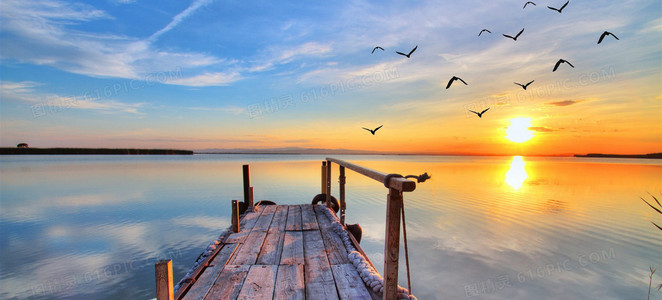
\includegraphics[width=0.8\textwidth]{image.jpeg}
        \captionof{figure}{A figure}
    \end{center}
\end{tex}

\begin{tex}
    \begin{center}
        \begin{tabular}{|c|c|c|}
            \hline
            a & b & c \\
            \hline
            a & b & c \\
            \hline
        \end{tabular}
        \captionof{table}{A table}
    \end{center}
\end{tex}

\begin{bluebox}
    \begin{center}
        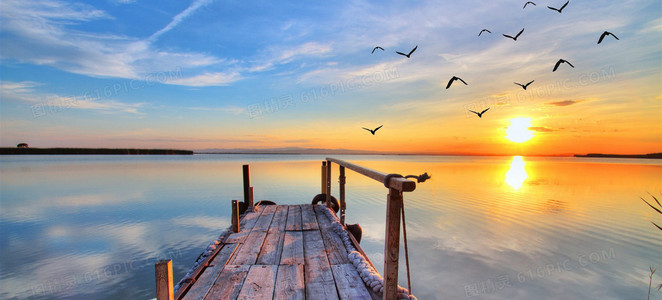
\includegraphics[width=0.8\textwidth]{image.jpeg}
        \captionof{figure}{A figure}
    \end{center}
    \begin{center}
        \begin{tabular}{|c|c|c|}
            \hline
            a & b & c \\
            \hline
            a & b & c \\
            \hline
        \end{tabular}
        \captionof{table}{A table}
    \end{center}
\end{bluebox}




% ------------------------------------------------------------------------------
\section{Code}
{\color{blue}We defined a code environment for the R language:}

\begin{R}
> a+1
# [1] 2
\end{R}

{\color{blue}If you use another language, modify the following code:}

\begin{tex}
\lstnewenvironment{R}{\lstset{
    language=R,
    basicstyle=\footnotesize\ttfamily,
    numbers=left,
    numberstyle=\tiny\color{black},
    stepnumber=1,
    numbersep=5pt,
    backgroundcolor=\color{mygray},
    showspaces=false,
    showstringspaces=false,
    showtabs=false,
    frame=single,
    rulecolor=\color{black},
    tabsize=4,
    captionpos=b,
    breaklines=true,
    breakatwhitespace=false,
    keywordstyle=\ttfamily\bfseries\color{myblue},
    commentstyle=\ttfamily\bfseries\color{myred},
    stringstyle=\ttfamily\bfseries\color{mygreen}
}}{}
\end{tex}

{\color{blue}The \verb|tex| environment was defined just for writing this tutorial. You can remove it if it's unnecessary.}







% ------------------------------------------------------------------------------
\section{Macros}

This template includes the macros shown in Tables \ref{table1} and \ref{table2}.


\begin{table}[h]
\centering
\setlength{\arrayrulewidth}{1pt} \setlength{\tabcolsep}{10pt}     \renewcommand{\arraystretch}{1.5} \begin{tabular}{|>{\centering\arraybackslash}m{3cm}|>{\centering\arraybackslash}m{3cm}||>{\centering\arraybackslash}m{3cm}|>{\centering\arraybackslash}m{3cm}|}
\hline
\textbf{Macro} & \textbf{Symbol} & \textbf{Macro} & \textbf{Symbol} \\
\hline
\texttt{\textbackslash C}  & $ \C $   & \texttt{\textbackslash ninfo\{a\}}    & $\ninfo{a}$ \\
\texttt{\textbackslash Q}  & $ \Q $   & \texttt{\textbackslash ninfc\{a\}}    & $\ninfc{a}$ \\
\texttt{\textbackslash Z}  & $ \Z $   & \texttt{\textbackslash pinfo\{a\}}    & $\pinfo{a}$ \\
\texttt{\textbackslash Rn\{k\}}  & $ \Rn{k} $   & \texttt{\textbackslash  pinfc\{a\}}    & $\pinfc{a}$ \\
\texttt{\textbackslash borel}  & $ \borel $   & \texttt{\textbackslash pa\{a,b,c\}}    & $\pa{a,b,c}$ \\
\texttt{\textbackslash familay}  & $ \family $   & \texttt{\textbackslash br\{a,b,c\}}    & $\br{a,b,c}$ \\
\texttt{\textbackslash oc\{a,b\}}  & $ \oc{a,b} $   & \texttt{\textbackslash cbr\{a,b,c\}}    & $\cbr{a,b,c}$ \\
\texttt{\textbackslash co\{a,b\}}  & $ \co{a,b} $   & \texttt{\textbackslash inner\{a,b\}}  & $ \inner{a,b} $  \\
\hline

 \texttt{\textbackslash norm\{a\}}    & $\norm{a}$ & \texttt{\textbackslash abs\{a\}}    & $\abs{a}$ \\
\texttt{\textbackslash floor\{a\}}  & $ \floor{a} $   & \texttt{\textbackslash ceil\{a\}}    & $\ceil{a}$ \\


\texttt{\textbackslash dd}  & $ \dd $   & \texttt{\textbackslash dv\{f\}\{x\}\{2\}}    & $\dv{f}{x}{2}$ \\
\texttt{\textbackslash p}  & $ \p $   & \texttt{\textbackslash pdv\{f\}\{x\}\{2\}}    & $\pdv{f}{x}{2}$ \\
  
\texttt{\textbackslash pr}  & $ \pr $   & \texttt{\textbackslash Cov}    & $\Cov$ \\
\texttt{\textbackslash E}   & $\E$   & \texttt{\textbackslash Corr}   & $\Corr$ \\
\texttt{\textbackslash I\{x>1\}} & $\I{x>1}$ & \texttt{\textbackslash inD} & $\inD$ \\
\texttt{\textbackslash inAS}   & $\inAS$ & \texttt{\textbackslash inP} & $\inP$ \\
\texttt{\textbackslash inLp}   & $\inLp$ & \texttt{\textbackslash inMSE} & $\inMSE$ \\
\hline

\verb|\simIND|&$\simIND$ & \verb|\indep|& $\indep$\\
\verb|\IID|& $\iid$ & \verb|\simIID| &$\simIID$\\
\verb|\mat{a&b\\c&d}|& $\mat{a&b\\c&d}$ &\verb|\smat{a&b\\c&d}|  &$\smat{a&b\\c&d}$\\
\verb|\bmat{a&b\\c&d}|& $\bmat{a&b\\c&d}$& \verb|\bsmat{a&b\\c&d}| & $\bsmat{a&b\\c&d}$\\
\verb|\pmat{a&b\\c&d}| & $\pmat{a&b\\c&d}$& \verb|\psmat{a&b\\c&d}| &$\psmat{a&b\\c&d}$\\
\verb|\argmin| & $\argmin$ &\verb|\argmax| & $\argmax$ \\
\hline
\end{tabular}
\caption{Macros and Corresponding Symbols for Math Operator}
\label{table1}
\end{table}
%% statistical notation
\begin{table}[h]
\centering
\setlength{\arrayrulewidth}{1pt} 
\setlength{\tabcolsep}{10pt}    
\renewcommand{\arraystretch}{1.5} 
\begin{tabular}{|>{\centering\arraybackslash}m{3cm}|>{\centering\arraybackslash}m{3cm}||>{\centering\arraybackslash}m{3cm}|>{\centering\arraybackslash}m{3cm}|}
\hline
\textbf{Macro} & \textbf{Symbol} & \textbf{Macro} & \textbf{Symbol} \\
\texttt{\textbackslash median}   & $\median$   & \texttt{\textbackslash Var}    & $\Var$ \\
\texttt{\textbackslash SD}  & $\SD$  & \texttt{\textbackslash CV}     & $\CV$ \\
\texttt{\textbackslash Bias}    & $\Bias$   & \texttt{\textbackslash AMSE}   & $\AMSE$ \\
\texttt{\textbackslash MSE} & $\MSE$  & \texttt{\textbackslash ARE}    & $\ARE$ \\
\texttt{\textbackslash AV}  & $\AV$  & \texttt{\textbackslash CRLB}   & $\CRLB$ \\
\texttt{\textbackslash TN} & $\TN$ & \texttt{\textbackslash Bern} & $\Bern$ \\
\texttt{\textbackslash Unif} & $\Unif$ & \texttt{\textbackslash Normal} & $\Normal$ \\
\texttt{\textbackslash logNormal} & $\logNormal$ & \texttt{\textbackslash Bin} & $\Bin$ \\
\hline
\texttt{\textbackslash NB} & $\NB$ & \texttt{\textbackslash HG} & $\HG$ \\
\texttt{\textbackslash Geom} & $\Geom$ & \texttt{\textbackslash Beta} & $\Beta $ \\
\texttt{\textbackslash BetaBin} & $\BetaBin$ & \texttt{\textbackslash Ga} & $\Ga$ \\
\texttt{\textbackslash Exp} & $\Exp$ & \texttt{\textbackslash Expo} & $\Expo$ \\
\texttt{\textbackslash Po} & $\Po$ & \texttt{\textbackslash Multi} & $\Multi$ \\
\texttt{\textbackslash student} & $\student$ & \texttt{\textbackslash Cauchy} & $\Cauchy$ \\
\verb|\Pareto| & $\Pareto$ & \verb|\RV| & \RV \\
\verb|\Laplace| & $\Laplace$ & \verb|\cdf| & \cdf \\
\verb|\Logistic| & $\Logistic$ & \verb|\cgf| & \cgf \\
\verb|\Dir| & $\Dir$ & \verb|\pdf| & \pdf \\
\verb|\DP| & $\DP$ & \verb|\pmf| & \pmf \\
\verb|\Inv| & $\Inv$ & \verb|\chf| & \chf \\
\hline
\verb|\F| & $\F$ & \verb|\mgf| & \mgf \\
\verb|\EF| & $\EF$ & \verb|\MLE| & \MLE \\
\verb|\NEF| & $\NEF$ & \verb|\MAP| & \MAP \\
\verb|\Med| & \Med & \verb|\MME| & \MME \\
\verb|\EB| & $\EB$ & \verb|\QME| & \QME \\
\verb|\UMVUE| & \UMVUE & \verb|\MPT| & \MPT \\
\verb|\UMPT| & \UMPT & \verb|\LRT| & \LRT \\
\verb|\mis| & \mis & \verb|\obs| & \obs \\
\verb|\com| & \com & \verb|\MCMC| & \MCMC \\
\verb|\burn| & $\burn$ & \verb|\thin| & $\thin$ \\
\verb|\ESS| & $\ESS$ & & \\
\hline
\end{tabular}
\caption{Macros and Corresponding Symbols for Statistical Notation}
\label{table2}
\end{table}

\newpage



%----------------------------------------

% citations
%\bibliographystyle{plain}
%\bibliography{citations}
%\newpage
%\appendixname
%\appendix
\end{document}
